Given the above model, our goal is to find the maximum \emph{a posteriori} (MAP) spike train, i.e., the most likely spike train, $\bn_{MAP}$,  given the fluorescence measurements, $\bF$. Formally, we have:

\begin{align}
\bn_{MAP} &=  \anx P[\bn | \bF] =  \anx \frac{1}{P[\bF]} P[\bF | \bn] P[\bn] =  \anx  P[\bF | \bn] P[\bn]   \label{eq:nhat1} %\\
\end{align}

\noindent where $n_t$ is constrained to be an integer ($\mathbb{N}_0=\{0,1,2,\ldots\}$), the second equality follows from two applications of Bayes rule, and the third equality follows because $P[\bF]$ merely scales the results, but does not change the relative quality of various spike trains.  A careful analysis of the above model, Eqs. \eqref{eq:F}--\eqref{eq:n}, suggests that we have a \emph{state-space model} \cite{DurbinKoopman01}:

\begin{subequations} \label{eq:ssm}
\begin{align} 
F_t &= \alpha (C_t + \beta) + \sig \varepsilon_t, \qquad& \varepsilon_t \overset{iid}{\sim} \mN(0,1) \\
C_t &= \gam C_{t-1} + n_t, & n_t \overset{iid}{\sim} \text{Poiss}(\lam \Del)
\end{align}
\end{subequations}

\noindent where $\gam = 1-\tau/\Del$, and $n_t$ has been rescaled appropriately.  We use the above formulation to simplify Eq. \eqref{eq:nhat1}:

\begin{subequations}  \label{eq:obj}
\begin{align}
\bn_{MAP}
&= \argmax_{n_t \in \mathbb{N}_0 \forall t} \prod_{t=1}^T  P[F_t | C_t]  P[C_t | C_{t-1}]  \label{eq:nhat2} \\
&= \argmax_{n_t \in \mathbb{N}_0 \forall t} \prod_{t=1}^T  P[F_t | C_t]  P[n_t] 
%\label{eq:nhat2}
= \argmax_{n_t \in \mathbb{N}_0 \forall t} \sum_{t=1}^T \big( \log P[F_t | C_t] + \log P[n_t]\big)  \label{eq:nhat2} %\\
%&= \ann  \sum_{t=1}^T \bigg( \frac{1}{2 \sig^2}(F_t - \alpha(C_t + \beta))^2  -  n_t \log \lam \Del + \log n_t! \bigg), \label{eq:nhat4}   
\end{align} 
\end{subequations}

\noindent where Eq. \eqref{eq:nhat1} follows from Eq. \eqref{eq:ssm}, and Eq. \eqref{eq:nhat2} follows from Eq. \eqref{eq:C}. Plugging Eqs. \eqref{eq:F} and \eqref{eq:n} into Eq. \eqref{eq:nhat2} yields:

\begin{align} \label{eq:MAP}
\bn_{MAP} &= \ann  \sum_{t=1}^T \bigg( \frac{1}{2 \sig^2}(F_t - \alpha(C_t + \beta))^2  -  n_t \log \lam \Del + \log n_t! \bigg), 
\end{align} 

\noindent Unfortunately, solving Eq. \eqref{eq:MAP} exactly is computationally intractable, as it requires a nonlinear search over an infinite number of  possible spike trains.  We could restrict our search space by imposing an upper bound, $k$, on the number of spikes within a frame.  However, in that case, the computational complexity scales \emph{exponentially} with the number of image frames --- more specifically, requires $O(k^T)$ time --- which for pragmatic reasons is intractable.  Thus, we approximate Eq. \eqref{eq:MAP}, by modifying Eq. \eqref{eq:C}, replacing the Poisson distribution with one that yields a log-concave problem.  This reduces the algorithmic complexity from requiring a search over $O(k^T)$ possible spike trains, to polynomial complexity, i.e., $O(T^p)$, where $p$ depends on the precise details of the algorithm.  

Two distributions naturally arise as possible approximations to a Poisson: (i) exponential, and (ii) Gaussian.  As depicted in Figure \ref{fig:dist_comp}  an exponential distribution (dashed gray line) is an excellent approximation to the Poisson distribution (solid black line), when $\lam$ is small (left panel).  On the other hand, when $\lam$ is large, a Gaussian distribution (dash-dotted gray line) closely approximates a Poisson when $\lam$ is large (right panel). Thus, \nai vely, it seems as though it may be desirable to use a Gaussian approximation when the neuron is firing with a high firing rate, and approximate the Poisson with an exponential when the neuron is firing sparsely.  The Wiener filter is, in fact, the optimal filter given the Gaussian approximation \cite{Wiener49} (see \cite{HolekampHoly08} for an application of the Wiener filter to this problem).  Below, we develop an algorithm to perform inference given the exponential distribution.  

\begin{figure}[H]
\centering 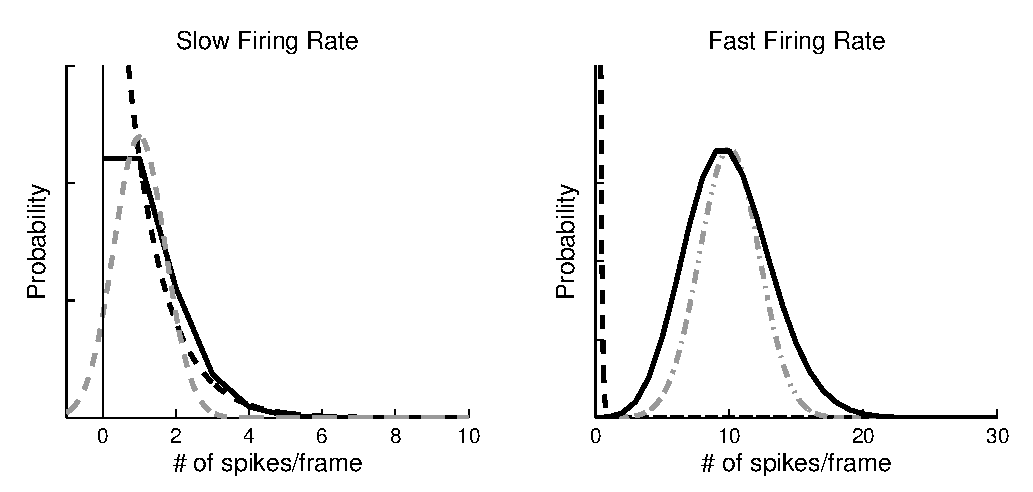
\includegraphics[width=.9\linewidth]{../figs/dist_comp}
\caption{Approximating a Poisson distribution.  Left panel: when $\lam$ is small (e.g., $\approx 1$), an exponential distribution (dashed gray line) approximates the Poisson distribution (solid black line) well, but a Gaussian distribution (dash-dotted gray line) does not.  Right panel: when $\lam$ is large (e.g., $\approx 20$), the inverse is true.} \label{fig:dist_comp}
\end{figure}